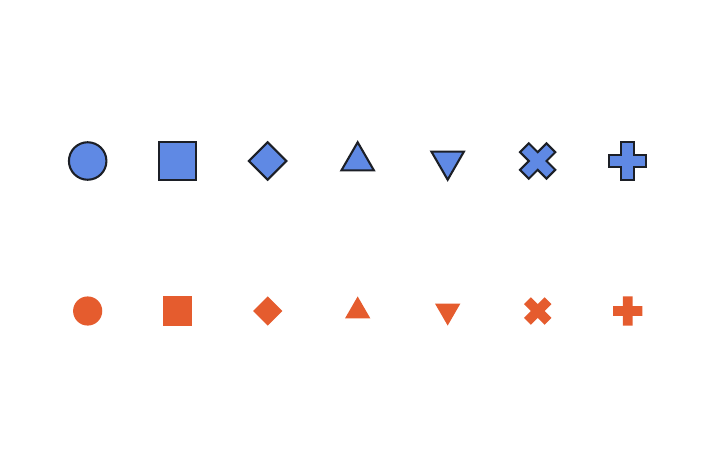
\begin{tikzpicture}[every node/.style={inner sep=0bp,outer sep=0bp}]
  \def\quivermarkA#1#2{\path[fill,draw,shift={(#1,#2)}] (0bp,0bp) circle[radius=6.75bp];}
  \definecolor{qcB}{rgb}{0.16,0.38,0.86}
  \definecolor{qcC}{rgb}{0.11,0.12,0.15}
  \def\quivermarkD#1#2{\path[fill,shift={(#1,#2)}] (0bp,0bp) circle[radius=5.25bp];}
  \definecolor{qcE}{rgb}{0.9,0.36,0.18}
  \def\quivermarkF#1#2{\path[fill,draw,shift={(#1,#2)}] (-6.75bp,-6.75bp) rectangle (6.75bp,6.75bp);}
  \def\quivermarkG#1#2{\path[fill,shift={(#1,#2)}] (-5.25bp,-5.25bp) rectangle (5.25bp,5.25bp);}
  \def\quivermarkH#1#2{\path[fill,draw,shift={(#1,#2)}] (0bp,-6.75bp) -- (6.75bp,0bp) -- (0bp,6.75bp) -- (-6.75bp,0bp) -- cycle;}
  \def\quivermarkI#1#2{\path[fill,shift={(#1,#2)}] (0bp,-5.25bp) -- (5.25bp,0bp) -- (0bp,5.25bp) -- (-5.25bp,0bp) -- cycle;}
  \def\quivermarkJ#1#2{\path[fill,draw,shift={(#1,#2)}] (0bp,6.75bp) -- (-5.846bp,-3.375bp) -- (5.846bp,-3.375bp) -- cycle;}
  \def\quivermarkK#1#2{\path[fill,shift={(#1,#2)}] (0bp,5.25bp) -- (-4.547bp,-2.625bp) -- (4.547bp,-2.625bp) -- cycle;}
  \def\quivermarkL#1#2{\path[fill,draw,shift={(#1,#2)}] (0bp,-6.75bp) -- (5.846bp,3.375bp) -- (-5.846bp,3.375bp) -- cycle;}
  \def\quivermarkM#1#2{\path[fill,shift={(#1,#2)}] (0bp,-5.25bp) -- (4.547bp,2.625bp) -- (-4.547bp,2.625bp) -- cycle;}
  \def\quivermarkN#1#2{\path[fill,draw,shift={(#1,#2)}] (3.182bp,-6.364bp) -- (6.364bp,-3.182bp) -- (3.182bp,0bp) -- (6.364bp,3.182bp) -- (3.182bp,6.364bp) -- (0bp,3.182bp) -- (-3.182bp,6.364bp) -- (-6.364bp,3.182bp) -- (-3.182bp,0bp) -- (-6.364bp,-3.182bp) -- (-3.182bp,-6.364bp) -- (0bp,-3.182bp) -- cycle;}
  \def\quivermarkO#1#2{\path[fill,shift={(#1,#2)}] (2.475bp,-4.95bp) -- (4.95bp,-2.475bp) -- (2.475bp,0bp) -- (4.95bp,2.475bp) -- (2.475bp,4.95bp) -- (0bp,2.475bp) -- (-2.475bp,4.95bp) -- (-4.95bp,2.475bp) -- (-2.475bp,0bp) -- (-4.95bp,-2.475bp) -- (-2.475bp,-4.95bp) -- (0bp,-2.475bp) -- cycle;}
  \def\quivermarkP#1#2{\path[fill,draw,shift={(#1,#2)}] (-2.25bp,-6.75bp) -- (2.25bp,-6.75bp) -- (2.25bp,-2.25bp) -- (6.75bp,-2.25bp) -- (6.75bp,2.25bp) -- (2.25bp,2.25bp) -- (2.25bp,6.75bp) -- (-2.25bp,6.75bp) -- (-2.25bp,2.25bp) -- (-6.75bp,2.25bp) -- (-6.75bp,-2.25bp) -- (-2.25bp,-2.25bp) -- cycle;}
  \def\quivermarkQ#1#2{\path[fill,shift={(#1,#2)}] (-1.75bp,-5.25bp) -- (1.75bp,-5.25bp) -- (1.75bp,-1.75bp) -- (5.25bp,-1.75bp) -- (5.25bp,1.75bp) -- (1.75bp,1.75bp) -- (1.75bp,5.25bp) -- (-1.75bp,5.25bp) -- (-1.75bp,1.75bp) -- (-5.25bp,1.75bp) -- (-5.25bp,-1.75bp) -- (-1.75bp,-1.75bp) -- cycle;}
  \useasboundingbox (0bp,0bp) rectangle (240bp,150bp);
  \begin{scope}[fill=qcB,fill opacity=0.75,draw=qcC,line width=0.75bp]
    \quivermarkA{21.6bp}{102bp}
  \end{scope}
  \begin{scope}[fill=qcE]
    \quivermarkD{21.6bp}{48bp}
  \end{scope}
  \begin{scope}[fill=qcB,fill opacity=0.75,draw=qcC,line width=0.75bp]
    \quivermarkF{54bp}{102bp}
  \end{scope}
  \begin{scope}[fill=qcE]
    \quivermarkG{54bp}{48bp}
  \end{scope}
  \begin{scope}[fill=qcB,fill opacity=0.75,draw=qcC,line width=0.75bp]
    \quivermarkH{86.4bp}{102bp}
  \end{scope}
  \begin{scope}[fill=qcE]
    \quivermarkI{86.4bp}{48bp}
  \end{scope}
  \begin{scope}[fill=qcB,fill opacity=0.75,draw=qcC,line width=0.75bp]
    \quivermarkJ{118.8bp}{102bp}
  \end{scope}
  \begin{scope}[fill=qcE]
    \quivermarkK{118.8bp}{48bp}
  \end{scope}
  \begin{scope}[fill=qcB,fill opacity=0.75,draw=qcC,line width=0.75bp]
    \quivermarkL{151.2bp}{102bp}
  \end{scope}
  \begin{scope}[fill=qcE]
    \quivermarkM{151.2bp}{48bp}
  \end{scope}
  \begin{scope}[fill=qcB,fill opacity=0.75,draw=qcC,line width=0.75bp]
    \quivermarkN{183.6bp}{102bp}
  \end{scope}
  \begin{scope}[fill=qcE]
    \quivermarkO{183.6bp}{48bp}
  \end{scope}
  \begin{scope}[fill=qcB,fill opacity=0.75,draw=qcC,line width=0.75bp]
    \quivermarkP{216bp}{102bp}
  \end{scope}
  \begin{scope}[fill=qcE]
    \quivermarkQ{216bp}{48bp}
  \end{scope}
\end{tikzpicture}
